\section{Model Analysis, Selection and Multiple Hypothesis Testing}
%\subsection*{Lecture 16}

%%%%%%%%%%%%%%%%%%%%%%%%%%%%%%%%%%%%%%%%%%%%%%%%%%%
\subsection{Model analysis}

Given a linear model, we can to some examination on the basis of visual analysis of residuals



\TODO{Example QQ plots ?}

\TODO{not homostochastic, not independent}
... transformed residuals free of trouble\dots
\TODO{long discussion of standardized / studentizes residuals ...}

%%%%%%%%%%%%%%%%%%%%%%%%%%%%%%%%%%%%%%%%%%%%%%%%%%%
\subsection{Model selection}
Some challenges when selecting model include:
\begin{enumerate}
    \item Unnecessary explanatory variables $\leadsto$ overfitting
    \item Missed relevant explanatory variables $\leadsto$ underfitting
    \item Quality of predictor $\centernot\iff$ Quality of estimator
\end{enumerate}

\TODO{example from 2017 exam}

Underfitting leads to biased estimation

Overfitting leads to greater variance in the estimators

%%%%%%%%%%%%%%%%%%%%%%%%%%%%%%%%%%%%%%%%%%%%%%%%%%%
%\subsection*{Lecture 17}
\subsubsection{Which model to choose}
Suppose $k$ covariates. Then we have $2^k$ possible models from maximal:
$$
    Y_i = \b_0+\b_1x_{i1} + \dots + \b_kx_{ik}.
$$
to minimal:
$$
    Y_i = \b_0.
$$
We want to arrive at a compromise between simplisity and goodness of fit. It is clear that the usual R2-score will not decrease by introducing additional variables, so we need to intruduce penalty for extra variables. Let $\sh^2$ be obtained from maximal model and $\mr{SSE}, p$ from the model of consideration.
\begin{enumerate}
    \item \term{Adjusted coefficient of determination}:
    $$
        \boxed{R^2_{\mr{adj}} = 1 - \frac{\mr{SSE} / (n-p-1)}{\mr{SST} / (n-1)} = 1 - (1-R^2)\frac{n-1}{n-p-1}}
    $$
    \item \term{Mallow's Cp parameter} (\hermetegn{Complexity parameter}):
    $$
        C_p = \frac{\mr{SSE}}{\sh^2} - n + 2p.
    $$
    \item \term{Akaibe information criterion}:
    $$
        \mr{AIC} = \frac{\mr{SSE}/n}{\sh^2} + 2\frac{p}{n}.
    $$
    \item \term{Bayesian information criterion}
    $$
        \mr{BIC} = \frac{\mr{SSE}/n}{\sh^2} + \ln{n}\frac{p}{n}.
    $$
\end{enumerate}
Note that for the 3 last options we want to minimise the statistic. In practice selection is done either with software or in to steps:
\begin{enumerate}
    \item For each $j=1,\dots,k$ choose the model with $j$ covariates of maximal R2-score. This gives $k$ models, so far not penalised.
    \item Consider these $k$ best models and choose `\hermetegn{best of the best} using one of the criteria. 
\end{enumerate}

%example...

%%%%%%%%%%%%%%%%%%%%%%%%%%%%%%%%%%%%%%%%%%%%%%%%%%%
%\subsection*{Lecture 18} % some 17
\subsection{Multiple hypothesis testing}
As before we consider the test:
$$
    \mr{H}_0 : \b_1=\dots=\b_k = 0.
$$
If this is now rejected, what about the individual tests $\b_j$? We can test individually using t-tests the hypothesis:
$$
    \mr{H}_0 : \b_j = 0.
$$
But if we have many parameters, $\p{\textrm{at least one type I error}}$ is large. In the worst case, for $m$ independent hypothesis we can compute this probability to be $1-(1-\alpha)^m$, which at significance $\alpha=0.05$ and $m=5, 20$ gives a probability $>0.22, >0.64$ respectivelly. We will now consider methods to resolve this issue. 
%The material is covered in more detail in \cite{Halle2017Multiple}.

%%%%%%%%%%%%%%%%%%%%%%%%%%%%%%%%%%%%%%%%%%%%%%%%%%%
\subsubsection{$p$-value is a random variable}

We recall that given an observation $t$ for the test statistiv $T$ we can compute the $p$-value, the probability of an equal of more extreme observation:
$$
    p(t) = \mathbb{P}_{\mathrm{H}_0} (T \geq t).
$$
Since $t$ is the observed value of a random variable, it is clear that the $p$-value is also random. The rejection criteria for $\mathrm{H}_0$ is: 
$$
    \mathrm{H}_0 \textrm{ is rejected} \Leftrightarrow p(t) \leq \alpha.
$$
An equivalent expression for the rejection criteria is:
$$
\mathrm{H}_0 \textrm{ is rejected} \Leftrightarrow t \geq t' \textrm{ with } \mathbb{P}_{\mathrm{H}_0} (T \geq t') = \alpha.    
$$
Hence we have
$$
    \mathbb{P}_{\mathrm{H}_0} (p(t) \leq \alpha) = \alpha,
$$
from which we conclude that under true $\mathrm{H}_0$, the $p$-value is uniformly distributed on $[0,1]$.

\begin{figure}[H]\centering
    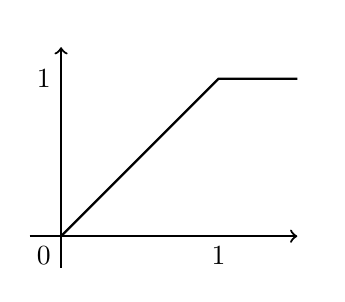
\begin{tikzpicture}[scale=2, thick]
        % Axes
        \draw[->, black] (-0.2, 0) -- (1.5, 0) node[right] {};
        \draw[->, black] (0, -0.2) -- (0, 1.2) node[above] {};
    
        % CDF
        \draw[thick] (0, 0) -- (1, 1) -- (1.5, 1);
    
        % Labels and ticks
        \draw (0, 0) node[below left] {0};
        \draw (1, 0) node[below] {1};
        \draw (1, 1) node[above right] {};
        \draw (0, 1) node[left] {1};
    
    \end{tikzpicture}
    \caption{Distribuon of the $p$-value.}
\end{figure}

%%%%%%%%%%%%%%%%%%%%%%%%%%%%%%%%%%%%%%%%%%%%%%%%%%%
\subsubsection{Testing $m$ hypothesis}
We begin by finding the $m$ $p$-values ($p_1,\dots,p_m$) corresponding to each hypothesis. We then need to choose the \term{local significance level} $\alpha_{\mr{loc}}$ and follow the rule that if $p$-value$\leq\alpha_{\mr{loc}}$ we reject the corresponding $\mr{H}_0$. We need to choose $\alpha_{\mr{loc}}$ such that the probability of at least one type I error is $\alpha$. The outcomes of our hypothesis test can be summarised by the table:
\begin{table}[htbp]
    \centering
    \caption{Multiple testing set-up}
    \begin{tabular}{cccc}
        \hline
         & H0 not rejected & H0 rejected & total \\
        \hline
        $\mr{H}_0$ true  & $U$   & $V$ & $m_0$\\
        $\mr{H}_0$ false & $T$   & $S$ & $m-m_0$\\
        total            & $m-R$ & $R$ & $m$\\
        \hline
    \end{tabular}
\end{table}
Note that we know $m$, the number of hypothesis, and the number $R$ of rejected hypothesis. Our goal is to control the \term{familywise error rate (FWER)}. This is the probability of at least one false positive finding:
$$
    \mr{FWER} = \p{V\geq 1} = 1- \p{V=0}.
$$
For independent hypothesis we find
\begin{align*}
    \mr{FWER} 
    &= 1- \p{p_1>\alpha_{\mr{loc}},\dots,p_m>\alpha_{\mr{loc}}}
    \\&= 1- \p{p_1>\alpha_{\mr{loc}}}\dots\p{p_m>\alpha_{\mr{loc}}}
    \\&= 1- (1-\alpha_{\mr{loc}})^m.
\end{align*}
If we for each hypothesis define the event:
$$
    R_j = \{\textrm{the j-th $\mr{H}_0$ is rejected but true}\} = \{p_j \leq \alpha_\mr{loc}\}.
$$
Then $\bar{R}_j=\{p_j > \alpha_{\mr{loc}}\}$ is the complementary event. We may write:
\begin{align*}
    \mr{FWER} 
    = \p{R_1\cup\dots\cup R_m} = 1 - \p{\bar{R}_1\cap\dots\cap \bar{R}_m}.
\end{align*}
We present two methods for choosing $\alpha_\mr{loc}$
\begin{enumerate}
    \item The \term{Bonferrony method} uses subadditivity to bound the $FWER$ by:
    $$
        \alpha = \mr{FWER} = \p{R_1\cup\dots\cup R_m} \leq \sum_{j=1}^m \p{R_j} = m \alpha_\mr{loc}.
    $$
    Hence the Bonferrony method is to let:
    \begin{equation}
        \boxed{\alpha_\mr{loc} = \frac{1}{m} \alpha}
    \end{equation}
    We make the following remarks:
    \begin{enumerate}
        \item This gives strong control (it works under any combination of true and false hypothesis).
        \item To get equality we need disjoint events / perfectly negativelly assosiated hypothesis.
        \item It is conservative: modelling dependencies may give lover requirement.
    \end{enumerate}
    \item For the \term{Šidák method} we make the assumption that we have \emph{independent tests}. Then we have seen that $\mr{FWER} = 1-(1-\alpha_{\mr{loc}})^m$. Hence the method is:
    \begin{equation}
        \boxed{\alpha_{\mr{loc}} = 1-(1-\alpha)^{1/m}}
    \end{equation}
    Again, we have strong control. The estimate is also exact when the tests are independent. It is conservative for positivelly dependent tests and liberal for negatively dependent tests. It is possible to show that the Šidák correction is always greater that the Bonferrony correction, so it is slighly less conservative; but we need to assume independence for exactness. 
\end{enumerate}

% ...
% example 2019 
% \dots
% example 2020
